\documentclass[../../thesis.tex]{subfiles}

\graphicspath{{./img/}}



\begin{document}


\section{Motifs in the Bitcoin Transaction Temporal Network}
\label{sec:motifs_bitcoin}


In the previous section, we showed a method for analyzing temporal networks. In Section~\ref{sec:bitcoin_as_a_graph} we showed a procedure to model the bitcoin transaction data as a temporal graph. To combine these two results, we start by downloading the Bitcoin transaction data from \url{https://blockchain.info/api/blockchain_api}. Using this API, we were able to download the raw JSON data of all the transactions between \textit{5 January 2017} and \textit{12 August 2017}, totalling 220 days of transactions. For each day of raw data, we follow the method proposed in section \ref{sec:bitcoin_as_a_graph} to obtain the temporal network of the Bitcoin transactions. The outcome is a collection of 220 files, where each file is a list of temporal edges, which represent the temporal network (see Definition~\ref{def:temporal_graph}). Afterwards, we run the Algorithm~\ref{sec:motifs_couting} for each Bitcoin temporal network day file, with parameter $\delta=3600$ seconds, as Subsection~\ref{sec:motifs_couting} describes. 


In order to describe the network, we calculated the number of nodes, number of edges, and number of triangles over time. Resulting in three time-series. Figure \ref{fig:number_nodes_by_time_chart} shows the number of nodes in our dataset, from 220 days, the maximum number of nodes is 940,446 on 23 May, the minimum 482,455 on 1 August, and average 697,657. 
 
 Sequentially, Figure~\ref{fig:number_edges_by_time_chart} shows the number of edges with as a maximum 3,092,194 on 11 August, a minimum of 960,204 on 15 January and 1 August as third lowest, and an average of 1,647,875. Lastly, Figure~\ref{fig:number_triangles_by_time_chart} shows the number of triangle motifs where the maximum is 3,887,064 on 4 August, the minimum 114,873 on 1 August, and with average 735,590. From our dataset, we can see 1 August is the day with the lowest usage of the Bitcoin protocol. 


\begin{figure}[H]
\centering
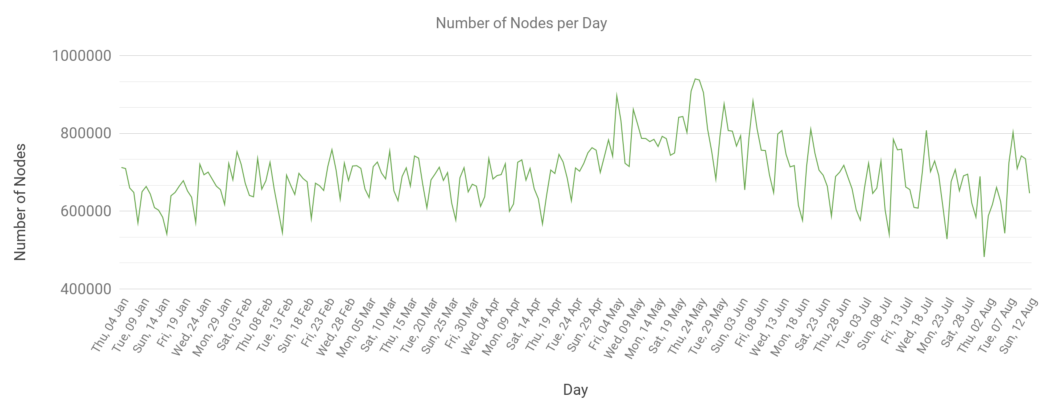
\includegraphics[width=1\textwidth]{content/unveiling/img/number_nodes_by_time_chart}
\caption{Time-series of the number of nodes computed from our bitcoin dataset. The maximum number of nodes is 940,446 on 23 May, the minimum 482,455 on 1 August, and average 697,657 nodes.}
\label{fig:number_nodes_by_time_chart}
\end{figure}


\begin{figure}[H]
\centering
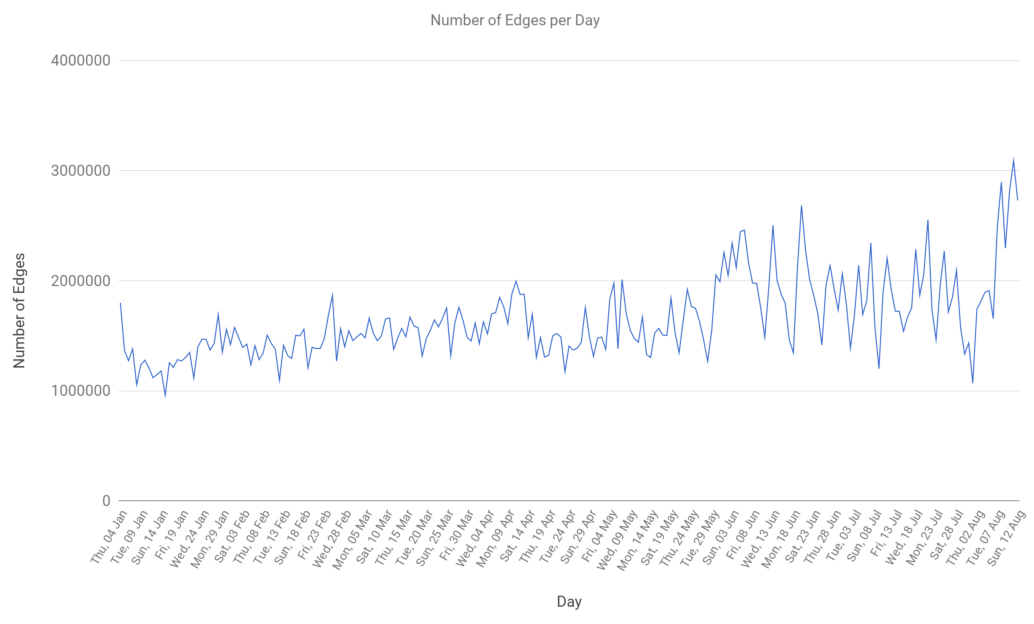
\includegraphics[width=\textwidth]{content/unveiling/img/number_edges_by_time_chart}
\caption{Time-series of the number of edges computed from our bitcoin dataset. The number of edges with maximum 3,092,194 on 11 August, the minimum 960,204 on 15 January and 1 August as third lowest, and average 1,647,875 edges. }
\label{fig:number_edges_by_time_chart}
\end{figure}


\begin{figure}[H]
\centering
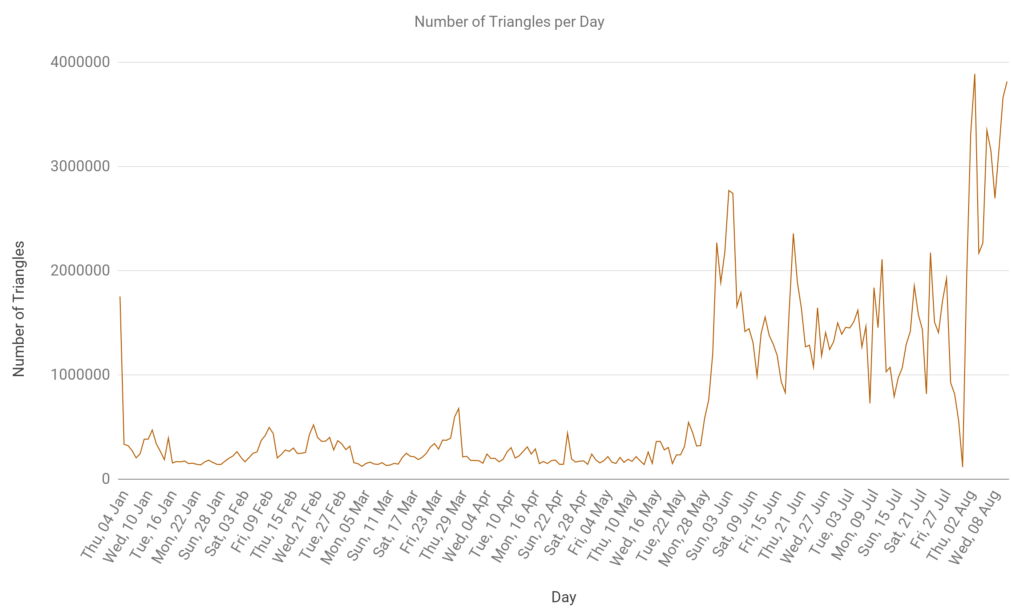
\includegraphics[width=\textwidth]{content/unveiling/img/number_triangles_by_time_chart}
\caption{Time-series of the number of triangles computed from our bitcoin dataset. The maximum is 3,887,064 on 4 August, the minimum 114,873 on 1 August, and with average 735,590 triangles.}
\label{fig:number_triangles_by_time_chart}
\end{figure}


Lastly, we compute the temporal motifs by selecting 3 data samples. We found for day A) May 4 2017, the motifs $M_{4,3}$(star), $M_{3,3}$(cycle), $M_{4,4}$(cycle), $M_{3,4}$(star), $M_{4,1}$(star), $M_{2,1}$(star) were the most counted and  $M_{6,2}$(cycle 2-nodes) the less counted. For day B) June 16 2017, we resulted in $M_{6,6}$, $M_{5,4}$(cycle), $M_{5,6}$(cycle), $M_{6,4}$(star), $M_{1,1}$(star), $M_{1,2}$(cycle) as most counted and $M_{3,5}$(triangle) as less counted. Finally, for day C) August 1 2017, the most counted were motifs $M_{6,6}$(star), $M_{1,6}$(star), $M_{1,1}$(star), $M_{4,1}$(star), $M_{4,3}$(star), $M_{6,3}$(star) and less counted was $M_{3,5}$(triangle), as it was in day B) as well. Note here that triangles motifs were never high counted. 

Our attention in this work is how the temporal motifs in the Bitcoin transactions temporal network \textit{change over time}. For that reason, our analysis is solely over subgraphs by days. Lastly, we normalize our motifs counts data. For better visualization of the behavior of the motifs, we compute the variance of the motifs and selected 6 highest variance motifs: $M_{1,6}$,$M_{6,6}$, $M_{1,1}$, $M_{2,5}$, $M_{1,5}$ and $M_{2,6}$. Surprisingly, the motifs with highest variance had a significant increase at the end of May 2017, as we can see the first plateau, and a vital increase, the second plateau, around August 2017 in its counts as Figure~\ref{fig:1h_temporalmotif_by_time_series_all} shows. We can infer that: those days precisely match with meaningful changes to the Bitcoin protocol. Accurately, on 22 May 2017, the \href{https://github.com/bitcoin/bips/blob/master/bip-0091.mediawiki}{Bitcoin Implementation Proposal Number 91} was created. This proposal, allows the Bitcoin miners to agree or not to the new changes on the Bitcoin protocol, having until 15 November 2017 to decide. Furthermore, on 1 August 2017, the motifs accurately capture a modification of the network. On that day, the first Bitcoin break of consensus happened [\href{https://www.cnbc.com/2017/07/31/blockchain-fork-will-create-new-digital-crypto-currency-bitcoin-cash.html}{1}, \href{https://www.theverge.com/2017/8/1/16075276/bitcoin-cash-hard-fork-coinbase}{2}, \href{https://motherboard.vice.com/en_us/article/9kwepa/bitcoin-has-forked}{3}, \href{https://techcrunch.com/2017/08/02/wtf-is-bitcoin-cash-and-is-it-worth-anything/}{4}, \href{http://money.cnn.com/2017/08/01/technology/business/bitcoin-cash-new-currency/index.html}{5}], which ended in the split of the Bitcoin Blockchain into two parallels Blockchains, this is the reflex of the mining nodes not finding a consensus among them, where some of them agreed and some other disagreed, on the rules proposed on 22 May 2017. Thus, resulting in rupture of the Blockchain. This action produced a second cryptocurrency sibling of the Bitcoin, called Bitcoin Cash. Additionally, this change on the protocol pushed a halt on several Cryptocurrencies Exchanges, and Wallets. These reasons can explain why 1 August was the day with the lowest usage of the Bitcoin protocol.



\begin{figure}
\centering
\includegraphics[width=\textwidth]{content/unveiling/img/topmotifs_lines.pdf}
\caption{Time series from all dates chart of the 6 highest variance motifs: $M_{1,6}$,$M_{6,6}$, $M_{1,1}$, $M_{2,5}$, $M_{1,5}$ and $M_{2,6}$ counts over the Bitcoin transaction temporal network. The red lines mark the exactly dates with meaningful changes on the Bitcoin Protocol: 22 May 2017 the \href{https://github.com/bitcoin/bips/blob/master/bip-0091.mediawiki}{Bitcoin Implementation Proposal Number 91} activation allowing the Bitcoin miners to agree or not to the new changes, and 1 August 2017 Bitcoin Cash creation [\href{https://www.cnbc.com/2017/07/31/blockchain-fork-will-create-new-digital-crypto-currency-bitcoin-cash.html}{1}, \href{https://www.theverge.com/2017/8/1/16075276/bitcoin-cash-hard-fork-coinbase}{2}, \href{https://motherboard.vice.com/en_us/article/9kwepa/bitcoin-has-forked}{3}, \href{https://techcrunch.com/2017/08/02/wtf-is-bitcoin-cash-and-is-it-worth-anything/}{4}, \href{http://money.cnn.com/2017/08/01/technology/business/bitcoin-cash-new-currency/index.html}{5}], where the miners did not agree on the new changes proposed on 22 May 2017. }
\label{fig:1h_temporalmotif_by_time_series_all}
\end{figure}

 Therefore, we conclude by showing empirical evidence that the temporal motifs proposed by \cite{temporalMotifs} were able to reveal fundamental structural changes of the Bitcoin transactions temporal network. Thus, confirming our intuition.



\end{document}